\ifx\wholebook\relax \else
% ------------------------ 

\documentclass{article}
%------------------- Other types of document example ------------------------
%
%\documentclass[twocolumn]{IEEEtran-new}
%\documentclass[12pt,twoside,draft]{IEEEtran}
%\documentstyle[9pt,twocolumn,technote,twoside]{IEEEtran}
%
%-----------------------------------------------------------------------------
%%
% loading packages
%
\newif\ifpdf
\ifx\pdfoutput\undefined % We're not running pdftex
  \pdffalse
\else
  \pdftrue
\fi
%
%
\ifpdf
  \RequirePackage[pdftex,%
            CJKbookmarks,%
       bookmarksnumbered,%
              colorlinks,%
          linkcolor=blue,%
              hyperindex,%
        plainpages=false,%
       pdfstartview=FitH]{hyperref}
\else
  \RequirePackage[dvipdfm,%
             CJKbookmarks,%
        bookmarksnumbered,%
               colorlinks,%
           linkcolor=blue,%
               hyperindex,%
         plainpages=false,%
        pdfstartview=FitH]{hyperref}
  \AtBeginDvi{\special{pdf:tounicode GBK-EUC-UCS2}} % GBK -> Unicode
\fi
\usepackage{hyperref}

% other packages
%-----------------------------------------------------------------------------
\usepackage{graphicx, color}
\usepackage{CJK}
%
% for programming 
%
\usepackage{verbatim}
\usepackage{listings}


\lstdefinelanguage{Smalltalk}{
  morekeywords={self,super,true,false,nil,thisContext}, % This is overkill
  morestring=[d]',
  morecomment=[s]{"}{"},
  alsoletter={\#:},
  escapechar={!},
  literate=
    {BANG}{!}1
    {UNDERSCORE}{\_}1
    {\\st}{Smalltalk}9 % convenience -- in case \st occurs in code
    % {'}{{\textquotesingle}}1 % replaced by upquote=true in \lstset
    {_}{{$\leftarrow$}}1
    {>>>}{{\sep}}1
    {^}{{$\uparrow$}}1
    {~}{{$\sim$}}1
    {-}{{\sf -\hspace{-0.13em}-}}1  % the goal is to make - the same width as +
    %{+}{\raisebox{0.08ex}{+}}1		% and to raise + off the baseline to match -
    {-->}{{\quad$\longrightarrow$\quad}}3
	, % Don't forget the comma at the end!
  tabsize=2
}[keywords,comments,strings]

\lstloadlanguages{C++, Lisp, Smalltalk}

% ======================================================================

\def\BibTeX{{\rm B\kern-.05em{\sc i\kern-.025em b}\kern-.08em
    T\kern-.1667em\lower.7ex\hbox{E}\kern-.125emX}}

\newtheorem{theorem}{Theorem}

%
% mathematics
%
\newcommand{\be}{\begin{equation}}
\newcommand{\ee}{\end{equation}}
\newcommand{\bmat}[1]{\left( \begin{array}{#1} }
\newcommand{\emat}{\end{array} \right) }
\newcommand{\VEC}[1]{\mbox{\boldmath $#1$}}

% numbered equation array
\newcommand{\bea}{\begin{eqnarray}}
\newcommand{\eea}{\end{eqnarray}}

% equation array not numbered
\newcommand{\bean}{\begin{eqnarray*}}
\newcommand{\eean}{\end{eqnarray*}}

\RequirePackage{CJK,CJKnumb,CJKulem,CJKpunct}
% we use CJK as default environment
\AtBeginDocument{\begin{CJK*}{GBK}{song}\CJKtilde\CJKindent\CJKcaption{GB}}
\AtEndDocument{\clearpage\end{CJK*}}

%
% loading packages
%
\newif\ifpdf
\ifx\pdfoutput\undefined % We're not running pdftex
  \pdffalse
\else
  \pdftrue
\fi
%
%
\ifpdf
  \RequirePackage[pdftex,%
       bookmarksnumbered,%
              colorlinks,%
          linkcolor=blue,%
              hyperindex,%
        plainpages=false,%
       pdfstartview=FitH]{hyperref}
\else
  \RequirePackage[dvipdfm,%
        bookmarksnumbered,%
               colorlinks,%
           linkcolor=blue,%
               hyperindex,%
         plainpages=false,%
        pdfstartview=FitH]{hyperref}
\fi
\usepackage{hyperref}

% other packages
%-----------------------------------------------------------------------------
\usepackage{graphicx, color}
%
% for programming 
%
\usepackage{verbatim}
\usepackage{listings}
\usepackage{algorithmic} %for pseudocode
\usepackage{algorithm}


\lstdefinelanguage{Smalltalk}{
  morekeywords={self,super,true,false,nil,thisContext}, % This is overkill
  morestring=[d]',
  morecomment=[s]{"}{"},
  alsoletter={\#:},
  escapechar={!},
  literate=
    {BANG}{!}1
    {UNDERSCORE}{\_}1
    {\\st}{Smalltalk}9 % convenience -- in case \st occurs in code
    % {'}{{\textquotesingle}}1 % replaced by upquote=true in \lstset
    {_}{{$\leftarrow$}}1
    {>>>}{{\sep}}1
    {^}{{$\uparrow$}}1
    {~}{{$\sim$}}1
    {-}{{\sf -\hspace{-0.13em}-}}1  % the goal is to make - the same width as +
    %{+}{\raisebox{0.08ex}{+}}1		% and to raise + off the baseline to match -
    {-->}{{\quad$\longrightarrow$\quad}}3
	, % Don't forget the comma at the end!
  tabsize=2
}[keywords,comments,strings]

\lstloadlanguages{C++, Lisp, Haskell, Python, Smalltalk}

% ======================================================================

\def\BibTeX{{\rm B\kern-.05em{\sc i\kern-.025em b}\kern-.08em
    T\kern-.1667em\lower.7ex\hbox{E}\kern-.125emX}}

\newtheorem{theorem}{Theorem}

%
% mathematics
%
\newcommand{\be}{\begin{equation}}
\newcommand{\ee}{\end{equation}}
\newcommand{\bmat}[1]{\left( \begin{array}{#1} }
\newcommand{\emat}{\end{array} \right) }
\newcommand{\VEC}[1]{\mbox{\boldmath $#1$}}

% numbered equation array
\newcommand{\bea}{\begin{eqnarray}}
\newcommand{\eea}{\end{eqnarray}}

% equation array not numbered
\newcommand{\bean}{\begin{eqnarray*}}
\newcommand{\eean}{\end{eqnarray*}}




\setcounter{page}{1}

\begin{document}

\fi
%--------------------------

% ================================================================
%                 COVER PAGE
% ================================================================

\title{Red-black tree, not so complex as it was thought}

\author{Liu~Xinyu
\thanks{{\bfseries Liu Xinyu } \newline
  Email: liuxinyu95@gmail.com \newline}
  }

\markboth{Red black tree}{AlgoXY}

\maketitle

\ifx\wholebook\relax
\chapter{Red-black tree, not so complex as it was thought}
\numberwithin{Exercise}{chapter}
\fi

% ================================================================
%                 Introduction
% ================================================================
\section{Introduction}
\label{introduction} \index{red-black tree}

\subsection{Exploit the binary search tree}
We have shown the power of binary search tree by using it to count
the occurrence of every word in Bible. The idea is to use binary
search tree as a dictionary for counting.

One may come to the idea that to feed a yellow page book
\footnote{A name-phone number contact list book} to a binary
search tree, and use it to look up the phone number for a contact.

By modifying a bit of the program for word occurrence counting
yields the following code.

\begin{lstlisting}
int main(int, char** ){
  ifstream f("yp.txt");
  map<string, string> dict;
  string name, phone;
  while(f>>name && f>>phone)
    dict[name]=phone;
  for(;;){
    cout<<"\nname: ";
    cin>>name;
    if(dict.find(name)==dict.end())
      cout<<"not found";
    else
      cout<<"phone: "<<dict[name];
  }
}
\end{lstlisting}

This program works well. However, if you replace the STL map 
with the binary search tree as mentioned previously, the 
performance will be bad, especially when you search some names such
as Zara, Zed, Zulu.

This is because the content of yellow page is typically listed
in lexicographic order. Which means the name list is in increase
order. If we try to insert a sequence of number 1, 2, 3, ..., n 
to a binary search tree. We will get a tree like in Figure \ref{fig:unbalanced-tree}.

\begin{figure}[htbp]
       \centering
	\includegraphics[scale=0.5]{img/unbalanced.ps}
        \caption{unbalanced tree} \label{fig:unbalanced-tree}
\end{figure}

This is a extreme unbalanced binary search tree. The looking up performs
$O(h)$ for a tree with height $h$. In balanced case, we benefit from 
binary search tree by $O(\lg N)$ search time. But in this extreme case, 
the search time downgraded to $O(N)$. It's no better than a normal link-list.

\begin{Exercise}

\begin{itemize}
\item For a very big yellow page list, one may want to speed up the
dictionary building process by two concurrent tasks (threads or processes).
One task reads the name-phone pair from the head of the list, while the
other one reads from the tail. The building terminates when these
two tasks meet at the middle of the list. What will be the binary
search tree looks like after building? What if you split the the
list more than two and use more tasks?

\item Can you find any more cases to exploit a binary search tree?
Please consider the unbalanced trees shown in figure 
\ref{fig:unbalanced-trees}.
\end{itemize}

\end{Exercise}

\begin{figure}[htbp]
       \centering
       \subfloat[]{\includegraphics[scale=0.5]{img/unbalanced-2.ps}} 
       \subfloat[]{\includegraphics[scale=0.5]{img/unbalanced-zigzag.ps}} \\
       \subfloat[]{\includegraphics[scale=0.5]{img/unbalanced-3.ps}}
       \caption{Some unbalanced trees} 
       \label{fig:unbalanced-trees}
\end{figure}

\subsection{How to ensure the balance of the tree}
In order to avoid such case, we can shuffle the input sequence by 
randomized algorithm, such as described in Section 12.4 in \cite{CLRS}.
However, this method doesn't always work, for example the input is fed 
from user interactively, and the tree need to be built/updated after each input.

There are many solutions people have ever found to make binary search tree balanced.
Many of them rely on the rotation operations to binary search tree. 
Rotation operations change the tree structure while maintain the ordering
of the elements. Thus it either improve or keep the balance property of the binary
search tree.

In this chapter, we'll first introduce about red-black tree, which is one of the 
most popular and widely used self-adjusting balanced 
binary search tree. In next chapter, we'll introduce about AVL tree, which is 
another intuitive solution; In later chapter about binary heaps, we'll show another 
interesting tree called splay tree, which can gradually adjust the the tree to make it
more and more balanced.

\subsection{Tree rotation}
\index{tree rotation}

\begin{figure}[htbp]
   \centering
   \setlength{\unitlength}{1cm}
   \begin{picture}(10, 4)
   \put(5, 2){$\Longleftrightarrow$}
   \subfloat[]{\includegraphics[scale=0.4]{img/rotate-r.ps}} 
   \subfloat[]{\includegraphics[scale=0.4]{img/rotate-l.ps}}
   \end{picture}
   \\
   \begin{picture}(1, 0.5)\end{picture} %pad
   \caption{Tree rotation, `rotate-left' transforms the tree from left side to right side, and `rotate-right' does the inverse transformation.} 
   \label{fig:tree-rotation}
\end{figure}

Tree rotation is a kind of special operation that can transform the tree structure
without changing the in-order traverse result. It based on the fact that
for a specified ordering, there are multiple binary search trees correspond to it.
Figure \ref{fig:tree-rotation} shows the tree rotation. For a binary search tree
on the left side, left rotate transforms it to the tree on the right, and right
rotate does the inverse transformation.

Although tree rotation can be realized in procedural way, there exists quite 
simple function description if using pattern matching.

\be
rotateL(T) = \left \{
  \begin{array}
  {r@{\quad:\quad}l}
  node(node(a, X, b), Y, c) & pattern(T) = node(a, X, node(b, Y, c)) \\
  T & otherwise
  \end{array}
\right .
\ee

\be
rotateR(T) = \left \{
  \begin{array}
  {r@{\quad:\quad}l}
  node(a, X, node(b, Y, c)) & pattern(T) = node(node(a, X, b), Y, c)) \\
  T & otherwise
  \end{array}
\right .
\ee

However, the pseudo code dealing imperatively has to set all fields accordingly.

\begin{algorithmic}[1]
\Function{Left-Rotate}{$T, x$}
  \State $p \gets$ \Call{Parent}{$x$}
  \State $y \gets$ \Call{Right}{$x$} \Comment{Assume $y \ne NIL$}
  \State $a \gets$ \Call{Left}{$x$}
  \State $b \gets$ \Call{Left}{$y$}
  \State $c \gets$ \Call{Right}{$y$}
  \State \Call{Replace}{$x, y$}
  \State \Call{Set-Children}{$x, a, b$}
  \State \Call{Set-Children}{$y, x, c$}
  \If{$p = NIL$}
    \State $T \gets y$
  \EndIf
  \State \Return $T$
\EndFunction

\Statex

\Function{Right-Rotate}{$T, y$}
  \State $p \gets$ \Call{Parent}{$y$}
  \State $x \gets$ \Call{Left}{$y$} \Comment{Assume $x \ne NIL$}
  \State $a \gets$ \Call{Left}{$x$}
  \State $b \gets$ \Call{Right}{$x$}
  \State $c \gets$ \Call{Right}{$y$}
  \State \Call{Replace}{$y, x$}
  \State \Call{Set-Children}{$y, b, c$}
  \State \Call{Set-Children}{$x, a, y$}
  \If{$p = NIL$}
    \State $T \gets x$
  \EndIf
  \State \Return $T$
\EndFunction

\Statex

\Function{Set-Left}{$x, y$}
  \State \Call{Left}{$x$} $\gets y$
  \If{$y \ne NIL$}
    \Call{Parent}{$y$} $\gets x$
  \EndIf
\EndFunction

\Statex

\Function{Set-Right}{$x, y$}
  \State \Call{Right}{$x$} $\gets y$
  \If{$y \ne NIL$}
    \Call{Parent}{$y$} $\gets x$
  \EndIf
\EndFunction

\Statex

\Function{Set-Children}{$x, L, R$}
  \State \Call{Set-Left}{$x, L$}
  \State \Call{Set-Right}{$x, R$}
\EndFunction

\Statex

\Function{Replace}{$x, y$}
  \If{\Call{Parent}{$x$} $= NIL$}
    \If{$y \ne NIL$}
      \Call{Parent}{$y$} $\gets NIL$
    \EndIf
  \ElsIf{\textproc{Left}(\Call{Parent}{$x$}) $= x$}
    \textproc{Set-Left}(\Call{Parent}{$x$}, $y$)
  \Else
    \textproc{Set-Right}(\Call{Parent}{$x$}, $y$)
  \EndIf
  \State \Call{Parent}{$x$} $\gets NIL$
\EndFunction
\end{algorithmic}

Compare these pseudo codes with the pattern matching functions, 
the former focus on the structure states changing, while the 
latter focus on the rotation process. As the title of this 
chapter indicated, red-black tree needn't be so complex as it 
was thought. Most traditional algorithm text books use the 
classic procedural way to teach red-black tree, there are 
several cases need to deal and all need carefulness to 
manipulate the node fields. However, by changing
the mind to functional settings, things get intuitive and
simple. Although there is some performance overhead.

Most of the content in this chapter is based on Chris Okasaki's
work in \cite{okasaki}.

% ================================================================
% Definition
% ================================================================
\section{Definition of red-black tree}
\index{red-black tree}

Red-black tree is a type of self-balancing binary search tree\cite{wiki}. 
\footnote{Red-black tree is one of the equivalent form of 2-3-4 tree (see chapter
B-tree about 2-3-4 tree). That is to say, for any 2-3-4 tree, there is at least 
one red-black tree has the same data order.} By using color changing and rotation, 
red-black tree provides a very simple and straightforward way to keep 
the tree balanced.

For a binary search tree, we can augment the nodes with a color field, a node
can be colored either red or black. We call a binary search tree red-black tree 
if it satisfies the following 5 properties\cite{CLRS}.
\index{red-black tree!red-black properties}

\begin{enumerate}
\item Every node is either red or black.
\item The root is black.
\item Every leaf (NIL) is black.
\item If a node is red, then both its children are black.
\item For each node, all paths from the node to descendant leaves contain the same number of black nodes.
\end{enumerate}

Why this 5 properties can ensure the red-black tree is well balanced? 
Because they have a key characteristic, the longest path from root to 
a leaf can't be as 2 times longer than the shortest path.

Please note the 4-th property, which means there won't be two adjacent 
red nodes. so the shortest path only contains black nodes, any paths 
longer than the shortest one has interval red nodes. According to 
property 5, all paths have the same number of black nodes, 
this finally ensure there won't be any path is 2 times longer than 
others\cite{wiki}. Figure \ref{fig:rbt-example} shows an example
red-black tree.

\begin{figure}[htbp]
       \begin{center}
	\includegraphics[scale=0.5]{img/rbt-example.ps}
        \caption{An example red-black tree} \label{fig:rbt-example}
       \end{center}
\end{figure}

All read only operations such as search, min/max are as same as in 
binary search tree. While only the insertion and deletion are special.

As we have shown in word occurrence example, many implementation of 
set or map container are based on red-black tree. One example is the 
C++ Standard library (STL)\cite{sgi-stl}. 

As mentioned previously, the only change in data layout is that
there is color information augmented to binary search tree.
This can be represented as a data field in imperative languages
such as C++ like below.

\lstset{language=C++}
\begin{lstlisting}
enum Color {Red, Black};

template <class T>
struct node{
  Color color;
  T key;
  node* left;
  node* right;
  node* parent;
};
\end{lstlisting}

In functional settings, we can add the color information
in constructors, below is the Haskell example of red-black tree
definition.

\lstset{language=Haskell}
\begin{lstlisting}
data Color = R | B
data RBTree a = Empty
              | Node Color (RBTree a) a (RBTree a)
\end{lstlisting}

\begin{Exercise}

\begin{itemize}
\item Can you prove that a red-black tree with $n$ nodes has
height at most $2 \lg (n+1)$?
\end{itemize}

\end{Exercise}

% ================================================================
%                 Insertion
% ================================================================
\section{Insertion}
\index{red-black tree!insertion}

Inserting a new node as what has been mentioned in binary search tree may 
cause the tree unbalanced. The red-black properties has to be maintained, 
so we need do some fixing by transform the tree after insertion.

When we insert a new key, one good practice is to always insert it as a 
red node. As far as the new inserted node isn't the root of the tree,
we can keep all properties except the 4-th one. that it may bring two 
adjacent red nodes.

Functional and procedural implementation have different fixing methods. 
One is intuitive but has some overhead, the other is a bit complex but has 
higher performance. Most text books about algorithm introduce the later
one. In this chapter, we focus on the former to show how easily a red-black 
tree insertion algorithm can be realized. The traditional procedural 
method will be given only for comparison purpose.

As described by Chris Okasaki, there are total 4 cases which violate property 4.
All of them has 2 adjacent red nodes. However, they have a uniformed form
after fixing\cite{okasaki} as shown in figure \ref{fig:insert-fix}. 

\begin{figure}[htbp]
   \begin{center}
     \setlength{\unitlength}{1cm}
     \begin{picture}(15, 15)
        % arrows
        \put(4.5, 9.5){\vector(1, -1){1}}
        \put(4.5, 5){\vector(1, 1){1}}
        \put(10, 9.5){\vector(-1, -1){1}}
        \put(10, 5){\vector(-1, 1){1}}
        % graphics
	\put(0, 7){\includegraphics[scale=0.5]{img/insert-ll.ps}}
        \put(0, 0){\includegraphics[scale=0.5]{img/insert-lr.ps}}
        \put(7, 7){\includegraphics[scale=0.5]{img/insert-rr.ps}}
        \put(8.5, 0){\includegraphics[scale=0.5]{img/insert-rl.ps}}
        \put(2, 5){\includegraphics[scale=0.5]{img/insert-fixed.ps}}
      \end{picture}
     \caption{4 cases for balancing a red-black tree after insertion} \label{fig:insert-fix}
  \end{center}
\end{figure}

Note that this transformation will move the redness one level up. 
So this is a bottom-up recursive fixing, the last step will make 
the root node red. According to property 2, root is always black. 
Thus we need final fixing to revert the root color to black. 

Observing that the 4 cases and the fixed result have strong pattern
features, the fixing function can be defined by using the similar 
method we mentioned in tree rotation. To avoid too long formula, 
we abbreviate $Color$ as $\mathcal{C}$, $Black$ as $\mathcal{B}$, and
$Red$ as $\mathcal{R}$.

\be
balance(T) = \left \{
  \begin{array}
  {r@{\quad:\quad}l}
  node(\mathcal{R}, node(\mathcal{B}, A, x, B), y, node(\mathcal{B}, C, z, D)) & match(T) \\
  T & otherwise
  \end{array}
\right .
\ee

where function $node()$ can construct a red-black tree node with 4 parameters 
as color, the left child, the key and the right child. Function $match()$
can test if a tree is one of the 4 possible patterns as the following.

\[
match(T) = \begin{array}{l}
         pattern(T) = node(\mathcal{B}, node(\mathcal{R}, node(\mathcal{R}, A, x, B), y, C), z, D) \lor \\
         pattern(T) = node(\mathcal{B}, node(\mathcal{R}, A, x, node(\mathcal{R}, B, y, C), z, D)) \lor \\
         pattern(T) = node(\mathcal{B}, A, x, node(\mathcal{R}, B, y, node(\mathcal{R}, C, z, D))) \lor \\ 
         pattern(T) = node(\mathcal{B}, A, x, node(\mathcal{R}, node(\mathcal{R}, B, y, C), z, D)) \\
         \end{array}
\]

With function $balance()$ defined, we can modify the previous binary search tree
insertion functions to make it work for red-black tree.

\be
insert(T, k) = makeBlack(ins(T, k))
\ee

where 

\be
ins(T, k) = \left \{
  \begin{array}
  {r@{\quad:\quad}l}
  node(\mathcal{R}, \phi, k, \phi) & T = \phi \\
  balance(node(ins(L, k), Key, R)) & k < Key \\
  balance(node(L, Key, ins(R, k))) & otherwise
  \end{array}
\right.
\ee 

$L, R, Key$ represent the left child, right child and the key of a tree.

\[
  \begin{array}{l}
  L = left(T) \\
  R = right(T) \\
  Key = key(T)
  \end{array}
\]


Function $makeBlack()$ is defined as the following, it forces the color
of a non-empty tree to be black.

\be
makeBlack(T) = node(\mathcal{B}, L, Key, R)
\ee

Summarize the above functions and use language supported pattern matching
features, we can come to the following Haskell program.

\lstset{language=Haskell}
\begin{lstlisting}
insert::(Ord a)=>RBTree a -> a -> RBTree a
insert t x = makeBlack $ ins t where
    ins Empty = Node R Empty x Empty
    ins (Node color l k r)
        | x < k     = balance color (ins l) k r
        | otherwise = balance color l k (ins r) --[3]
    makeBlack(Node _ l k r) = Node B l k r

balance::Color -> RBTree a -> a -> RBTree a -> RBTree a
balance B (Node R (Node R a x b) y c) z d = 
                Node R (Node B a x b) y (Node B c z d)
balance B (Node R a x (Node R b y c)) z d = 
                Node R (Node B a x b) y (Node B c z d)
balance B a x (Node R b y (Node R c z d)) = 
                Node R (Node B a x b) y (Node B c z d)
balance B a x (Node R (Node R b y c) z d) = 
                Node R (Node B a x b) y (Node B c z d)
balance color l k r = Node color l k r
\end{lstlisting} %$

Note that the 'balance' function is changed a bit from the original
definition. Instead of passing the tree, we pass
the color, the left child, the key and the right child to it.
This can save a pair of `boxing' and 'un-boxing' operations.

This program doesn't handle the case of inserting a duplicated key.
However, it is possible to handle it either by overwriting,
or skipping. Another option is to augment the data with a linked 
list\cite{CLRS}.

Figure \ref{fig:insert-example} shows two red-black trees
built from feeding list 11, 2, 14, 1, 7, 15, 5, 8, 4 and 1, 2, ..., 8.

\begin{figure}[htbp]
  \centering
  \includegraphics[scale=0.4]{img/insert-haskell.ps}
  \caption{insert results generated by the Haskell algorithm} \label{fig:insert-example}
\end{figure}

This algorithm shows great simplicity by summarizing the uniform feature
from the four different unbalanced cases. It is expressive over
the traditional tree rotation approach, that even in programming languages
which don't support pattern matching, the algorithm can still be
implemented by manually check the pattern. A Scheme/Lisp program
is available along with this book can be referenced as an example.

The insertion algorithm takes $O(\lg N)$ time to insert a key to
a red-black tree which has $N$ nodes.

\begin{Exercise}

\begin{itemize}
\item Write a program in an imperative language, such as
C, C++ or python to realize the same algorithm in this
section. Note that, because there is no language supported
pattern matching, you need to test the 4 different cases
manually.
\end{itemize}

\end{Exercise}

% ================================================================
%                 Deletion
% ================================================================

\section{Deletion}
\index{red-black tree!deletion}

Remind the deletion section in binary search tree. Deletion is 
`imperative only' for red-black tree as well. In typically
practice, it often builds the tree just one time, and 
performs looking up frequently after that. Okasaki explained
why he didn't provide red-black tree deletion in his work
in \cite{okasaki-blog}. One reason is that deletions are
much messier than insertions.

The purpose of this section is just to show that red-black
tree deletion is possible in purely functional settings, 
although it actually rebuilds the tree because trees are
read only in terms of purely functional data structure.
In real world, it's up to the user (or actually the 
programmer) to adopt the proper solution. One option is to mark
the node be deleted with a flag, and perform a tree rebuilding
when the number of deleted nodes exceeds 50\% of the total number
of nodes.

Not only in functional settings, even in imperative settings, 
deletion is more complex than insertion. We face more cases 
to fix. Deletion may also violate the red black tree properties,
so we need fix it after the normal deletion as described 
in binary search tree.

The deletion algorithm in this book are based on top of a
handout in \cite{lyn}. The problem only happens if you try to 
delete a black node, because it will violate the 4-th property 
of red-black tree, which means the number of black
node in the path may decreased so that it is not uniformed 
black-height any more.

When delete a black node, we can resume red-black property number
4 by introducing a 'doubly-black' concept\cite{CLRS}. It means
that the although the node is deleted, the blackness is kept
by storing it in the parent node. If the parent node is red,
it turns to black, However, if it has been already black, it
turns to `doubly-black'.

In order to express the 'doubly-black node', The definition
need some modification accordingly.

\lstset{language=Haskell}
\begin{lstlisting}
data Color = R | B | BB -- BB: doubly black for deletion
data RBTree a = Empty | BBEmpty -- doubly black empty
              | Node Color (RBTree a) a (RBTree a)
\end{lstlisting}

When deleting a node, we first perform the same deleting
algorithm in binary search tree mentioned in previous chapter.
After that, if the node to be sliced out is black, we 
need fix the tree to keep the red-black properties. Let's 
denote the empty tree as $\phi$, and for non-empty tree,
it can be decomposed to $node(Color, L, Key, R)$ for its
color, left sub-tree, key and the right sub-tree. The
delete function is defined as the following.

\be
delete(T, k) = blackenRoot(del(T, k))
\ee

where

\be
del(T, k) = \left \{
  \begin{array}
  {r@{\quad:\quad}l}
  \phi & T = \phi \\
  fixBlack^2(node(\mathcal{C}, del(L, k), Key, R)) & k < Key \\
  fixBlack^2(node(\mathcal{C}, L, Key, del(R, k))) & k > Key \\
  = \left \{
    \begin{array}{r@{\quad:\quad}l}
    mkBlk(R) & \mathcal{C} = \mathcal{B} \\
    R & otherwise
    \end{array} 
  \right. & L = \phi \\
  = \left \{ 
    \begin{array}{r@{\quad:\quad}l}
    mkBlk(L) & \mathcal{C} = \mathcal{B} \\
    L & otherwise
    \end{array} 
  \right.  & R = \phi \\
  fixBlack^2(node(\mathcal{C}, L, k', del(R, k'))) & otherwise 
  \end{array}
\right.
\ee

The real deleting happens inside function $del$. 
For the trivial case, that the tree is empty, the deletion
result is $\phi$; If the key to be deleted is less
than the key of the current node, we recursively 
perform deletion on its left sub-tree; if it is bigger
than the key of the current node, then we recursively
delete the key from the right sub-tree; Because it
may bring doubly-blackness, so we need fix it.

If the key to be deleted is equal to the key of the 
current node, we need splice it out. If one of its
children is empty, we just replace the node by
the other one and reserve the blackness of this
node. otherwise we cut and past the minimum 
element $k'=min(R)$ from the right sub-tree.

Function $delete$ just forces the result tree of $del$
to have a black root. This is realized by function
$blackenRoot$.

\be
blackenRoot(T) = \left \{
  \begin{array}
  {r@{\quad:\quad}l}
  \phi & T = \phi \\
  node(\mathcal{B}, L, Key, R) & otherwise \\
  \end{array}
\right .
\ee

Compare with the $makeBlack$ function, which is defined in 
red-black tree insertion section, they are almost same, 
except for the case of empty tree. This is only valid in 
deletion, because insertion can't result an empty tree, 
while deletion may.

Function $mkBlk$ is defined to reserved the blackness
of a node. If the node to be sliced isn't black, this function
won't be applied, otherwise, it turns a red node to black
and turns a black node to doubly-black. This function
also marks an empty tree to doubly-black empty.

\be
mkBlk(T) = \left \{
  \begin{array}
  {r@{\quad:\quad}l}
  \Phi & T = \phi \\
  node(\mathcal{B}, L, Key, R) & \mathcal{C} = \mathcal{R} \\
  node(\mathcal{B}^2, L, Key, R) & \mathcal{C} = \mathcal{B} \\
  T & otherwise
  \end{array}
\right .
\ee

where $\Phi$ means doubly-black empty node and $\mathcal{B}^2$
is the doubly-black color.

Summarizing the above functions yields the following Haskell
program.

\begin{lstlisting}
delete::(Ord a)=>RBTree a -> a -> RBTree a
delete t x = blackenRoot(del t x) where
    del Empty _ = Empty
    del (Node color l k r) x 
        | x < k = fixDB color (del l x) k r
        | x > k = fixDB color l k (del r x)
        -- x == k, delete this node
        | isEmpty l = if color==B then makeBlack r else r
        | isEmpty r = if color==B then makeBlack l else l
        | otherwise = fixDB color l k' (del r k') where k'= min r
    blackenRoot (Node _ l k r) = Node B l k r
    blackenRoot _ = Empty

makeBlack::RBTree a -> RBTree a
makeBlack (Node B l k r) = Node BB l k r -- doubly black
makeBlack (Node _ l k r) = Node B l k r
makeBlack Empty = BBEmpty
makeBlack t = t
\end{lstlisting}

The final attack to the red-black tree deletion algorithm is to
realize the $fixBlack^2$ function. The purpose of this function
is to eliminate the `doubly-black' colored node by rotation and
color changing.

Let's solve the doubly-black empty node first. For any node, 
If one of its child is doubly-black empty, and the other child is 
non-empty, we can safely replace the doubly-black empty with a 
normal empty node. 

Like figure \ref{fig:db-fix-1-nil}, if we
are going to delete the node 4 from the tree (Instead show the whole tree,
only part of the tree is shown), the program will use a doubly-black empty node
to replace node 4. In the figure, the doubly-black node is shown in black 
circle with 2 edges. It means that for node 5, it has a doubly-black empty 
left child and has a right non-empty child (a leaf node with key 6). In 
such case we can safely change the doubly-black empty to normal empty node. 
which won't violate any red-black properties.

\begin{figure}[htbp]
   \centering
   \subfloat[Delete 4 from the tree.]{\includegraphics[scale=0.4]{img/db-fix.ps}} \\
   \subfloat[After 4 is sliced off, it is doubly-black empty.]{\includegraphics[scale=0.4]{img/db-fix-1-nil-before.ps}}
   \subfloat[We can safely change it to normal NIL.]{\includegraphics[scale=0.4]{img/db-fix-1-nil-after.ps}}
   \caption{One child is doubly-black empty node, the other child is non-empty} \label{fig:db-fix-1-nil}
\end{figure}

On the other hand, if a node has a doubly-black empty node and the other child is
empty, we have to push the doubly-blackness up one level. For example in figure
\ref{fig:db-fix-2-nil}, if we want
to delete node 1 from the tree, the program will use a doubly-black empty node 
to replace 1. Then node 2 has a doubly-black empty node and has an empty right
node. In such case we must mark node 2 as doubly-black after change its
left child back to empty.

\begin{figure}[htbp]
   \centering
   \subfloat[Delete 1 from the tree.]{\includegraphics[scale=0.4]{img/db-fix.ps}} \\
   \subfloat[After 1 is sliced off, it is doubly-black empty.]{\includegraphics[scale=0.4]{img/db-fix-2-nil-before.ps}}
   \subfloat[We must push the doubly-blackness up to node 2.]{\includegraphics[scale=0.4]{img/db-fix-2-nil-after.ps}}
   \caption{One child is doubly-black empty node, the other child is empty.} \label{fig:db-fix-2-nil}
\end{figure}

Based on above analysis, in order to fix the doubly-black empty node, we define
the function partially like the following.

\be
fixBlack^2(T) = \left \{
  \begin{array}
  {r@{\quad:\quad}l}
  node(\mathcal{B}^2, \phi, Key, \phi) & (L = \phi \land R = \Phi) \lor (L = \Phi \land R = \phi) \\
  node(\mathcal{C}, \phi, Key, R) & L=\Phi \land R \neq \phi \\
  node(\mathcal{C}, L, Key, \phi) & R=\Phi \land L \neq \phi \\
  ... & ...
  \end{array}
\right .
\label{eq:db-nil}
\ee

After dealing with doubly-black empty node, we need to fix the case that the 
sibling of the doubly-black node is black and it has one red child. 
In this situation, we can fix the doubly-blackness with one rotation.
Actually there are 4 different sub-cases, all of them can be transformed
to one uniformed pattern. They are shown in the figure \ref{fig:del-case1}. 
These cases are described in \cite{CLRS} as case 3 and case 4.

\begin{figure}[htbp]
   \centering
   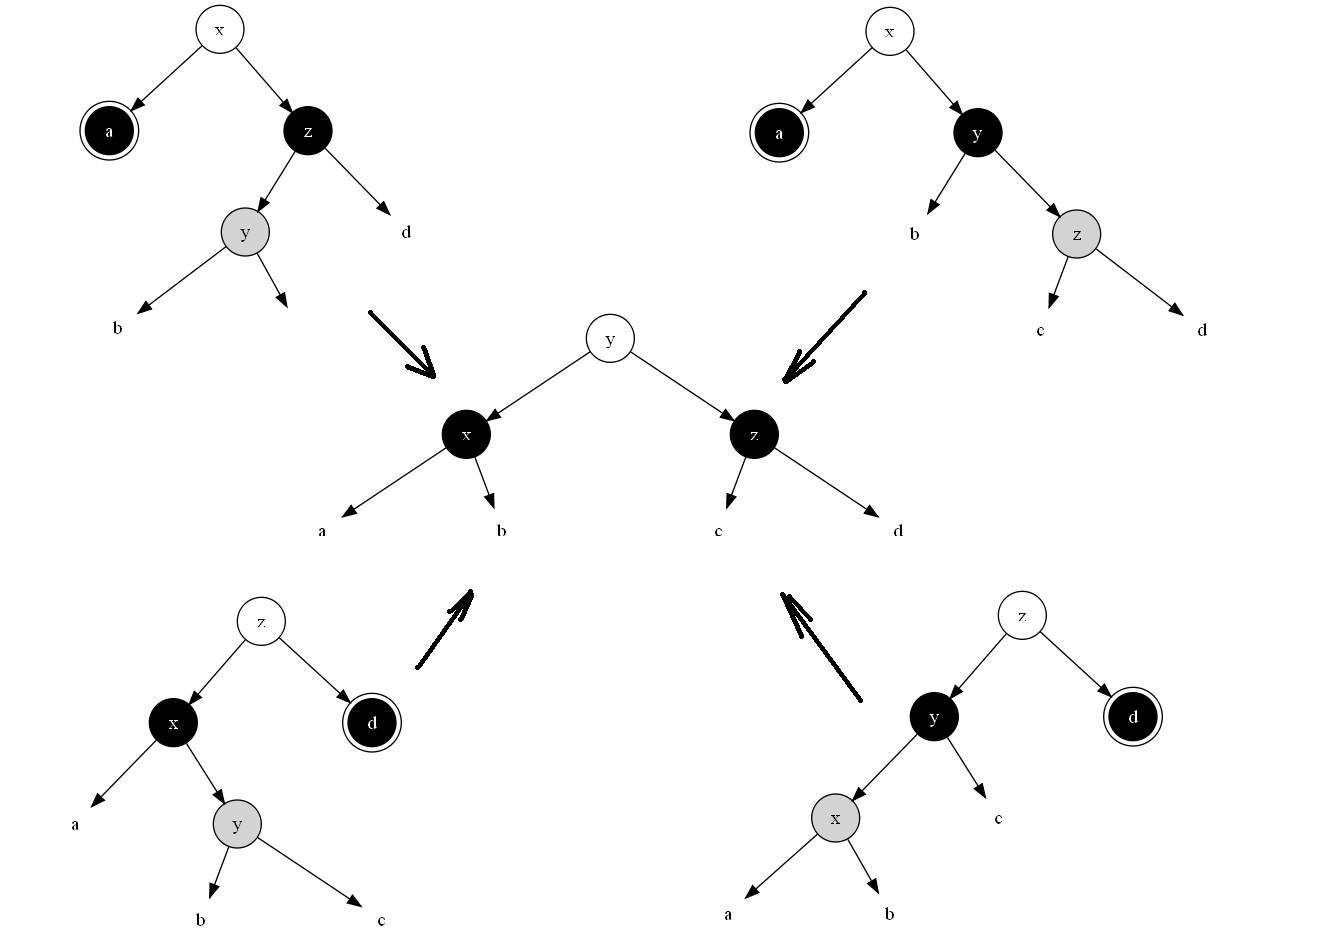
\includegraphics[scale=0.4]{img/del-case1.eps}
   \caption{Fix the doubly black by rotation, the sibling of the doubly-black node is black, and it has one red child.} \label{fig:del-case1}
\end{figure}

The handling of these 4 sub-cases can be defined on top of formula \ref{eq:db-nil}. 

\be
fixBlack^2(T) = \left \{
  \begin{array}
  {r@{\quad:\quad}l}
  ... & ... \\
  node(\mathcal{C}, node(\mathcal{B}, mkBlk(A), x, B), y, node(\mathcal{B}, C, z, D)) & p 1.1 \\
  node(\mathcal{C}, node(\mathcal{B}, A, x, B), y, node(\mathcal{B}, C, z, mkBlk(D))) & p 1.2 \\
  ... & ...
  \end{array}
\right .
\label{eq:db-case-1}
\ee

where $p 1.1$ and $p 1.2$ each represent 2 patterns as the following.

\[
p 1.1 = \left \{ \begin{array}{l}
  node(\mathcal{C}, A, x, node(\mathcal{B}, node(\mathcal{R}, B, y, C), z, D)) \land Color(A) = \mathcal{B}^2 \\
  \lor \\
  node(\mathcal{C}, A, x, node(\mathcal{B}, B, y, node(\mathcal{R}, C, z, D))) \land Color(A) = \mathcal{B}^2
  \end{array} \right \}
\]

\[
p 1.2 = \left \{ \begin{array}{l}
  node(\mathcal{C}, node(\mathcal{B}, A, x, node(\mathcal{R}, B, y, C)), z, D) \land Color(D) = \mathcal{B}^2 \\
  \lor \\
  node(\mathcal{C}, node(\mathcal{B}, node(\mathcal{R}, A, x, B), y, C), z, D) \land Color(D) = \mathcal{B}^2
  \end{array} \right \}
\]

Besides the above cases, there is another one that not only the sibling
of the doubly-black node is black, but also its two children are black. 
We can change the color of the sibling node to red; resume the 
doubly-black node to black and propagate the doubly-blackness one level 
up to the parent node as shown in figure \ref{fig:del-case2}. Note that
there are two symmetric sub-cases. This case is described in \cite{CLRS} 
as case 2.

\begin{figure}[htbp]
  \centering
  \setlength{\unitlength}{1cm}
  \begin{picture}(10, 4)
  \put(5, 2){$\Longrightarrow$}
  \subfloat[Color of $x$ can be either black or red.]{\includegraphics[scale=0.4]{img/case2-a.ps}}
  \subfloat[If $x$ was red, then it becomes black, otherwise, it becomes doubly-black.]{\includegraphics[scale=0.4]{img/case2-a1.ps}}
  \end{picture}
  \\
  \begin{picture}(10, 5)
  \put(5, 2){$\Longrightarrow$}
  \subfloat[Color of $y$ can be either black or red.]{\includegraphics[scale=0.4]{img/case2-b.ps}}
  \subfloat[If $y$ was red, then it becomes black, otherwise, it becomes doubly-black.]{\includegraphics[scale=0.4]{img/case2-b1.ps}}
  \end{picture}
  \\
  \begin{picture}(1, 0.5)\end{picture} %pad
  \caption{propagate the blackness up.} \label{fig:del-case2}
\end{figure}

We go on adding this fixing after formula \ref{eq:db-case-1}.

\be
fixBlack^2(T) = \left \{
  \begin{array}
  {r@{\quad:\quad}l}
  ... & ... \\
  mkBlk(node(\mathcal{C}, mkBlk(A), x, node(\mathcal{R}, B, y, C))) & p 2.1 \\
  mkBlk(node(\mathcal{C}, node(\mathcal{R}, A, x, B), y, mkBlk(C))) & p 2.2 \\
  ... & ...
  \end{array}
\right .
\label{eq:db-case-2}
\ee

where $p 2.1$ and $p 2.2$ are two patterns as below.

\[
p 2.1 = \left \{ \begin{array}{l}
  node(\mathcal{C}, A, x, node(\mathcal{B}, B, y, C)) \land \\
  Color(A) = \mathcal{B}^2 \land Color(B) = Color(C) = \mathcal{B}
  \end{array} \right \}
\]

\[
p 2.2 = \left \{ \begin{array}{l}
  node(\mathcal{C}, node(\mathcal{B}, A, x, B), y, C) \land \\
  Color(C) = \mathcal{B}^2 \land Color(A) = Color(B) = \mathcal{B}
  \end{array} \right \}
\]

There is a final case left, that the sibling of the doubly-black node is red.
We can do a rotation to change this case to pattern $p 1.1$ or $p 1.2$.
Figure \ref{fig:del-case3} shows about it.

\begin{figure}[htbp]
  \centering
  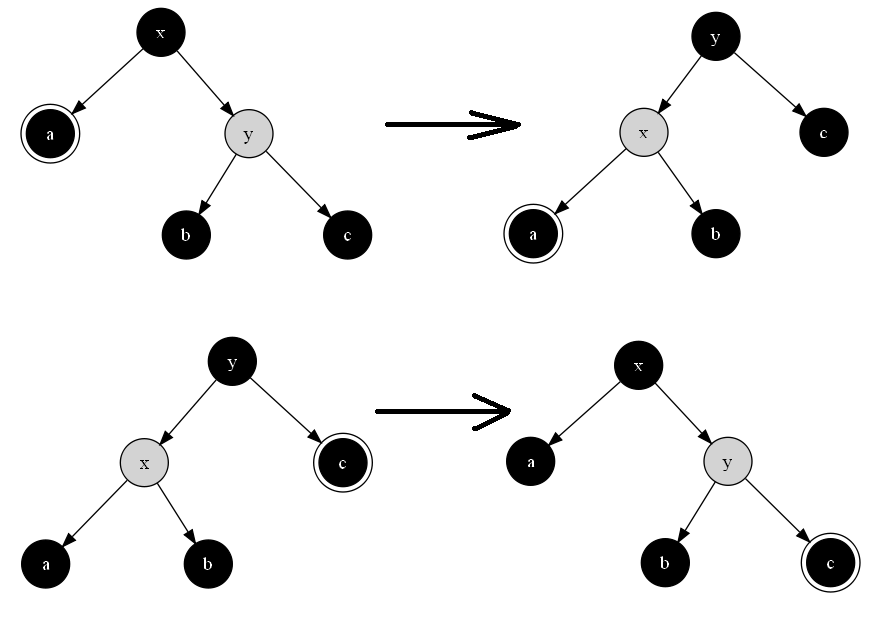
\includegraphics[scale=0.4]{img/del-case3.eps}
  \caption{The sibling of the doubly-black node is red.} \label{fig:del-case3}
\end{figure}

We can finish formula \ref{eq:db-case-2} with \ref{eq:db-case-3}.

\be
fixBlack^2(T) = \left \{
  \begin{array}
  {r@{\quad:\quad}l}
  ... & ... \\
  fixBlack^2(\mathcal{B}, fixBlack^2(node(\mathcal{R}, A, x, B), y, C) & p 3.1 \\
  fixBlack^2(\mathcal{B}, A, x, fixBlack^2(node(\mathcal{R}, B, y, C)) & p 3.2 \\
  T & otherwise
  \end{array}
\right .
\label{eq:db-case-3}
\ee

where $p 3.1$ and $p 3.2$ are two patterns as the following.

\[
p 3.1 = \{ Color(T) = \mathcal{B} \land Color(L) = \mathcal{B}^2 \land Color(R) = \mathcal{R} \}
\]

\[
p 3.2 = \{ Color(T) = \mathcal{B} \land Color(L) = \mathcal{R} \land Color(R) = \mathcal{B}^2 \}
\]


This two cases are described in \cite{CLRS} as case 1.

Fixing the doubly-black node with all above different cases is a recursive function. 
There are two termination conditions. One contains pattern $p 1.1$ and $p 1.2$, 
The doubly-black node was eliminated. The other cases may continuously propagate the 
doubly-blackness from bottom to top till the root.
Finally the algorithm marks the root node as black anyway. The doubly-blackness will be
removed.

Put formula \ref{eq:db-nil}, \ref{eq:db-case-1}, \ref{eq:db-case-2}, and \ref{eq:db-case-3}
together, we can write the final Haskell program.

\begin{lstlisting}
fixDB::Color -> RBTree a -> a -> RBTree a -> RBTree a
fixDB color BBEmpty k Empty = Node BB Empty k Empty
fixDB color BBEmpty k r = Node color Empty k r
fixDB color Empty k BBEmpty = Node BB Empty k Empty
fixDB color l k BBEmpty = Node color l k Empty
-- the sibling is black, and it has one red child
fixDB color a@(Node BB _ _ _) x (Node B (Node R b y c) z d) = 
      Node color (Node B (makeBlack a) x b) y (Node B c z d)
fixDB color a@(Node BB _ _ _) x (Node B b y (Node R c z d)) = 
      Node color (Node B (makeBlack a) x b) y (Node B c z d)
fixDB color (Node B a x (Node R b y c)) z d@(Node BB _ _ _) = 
      Node color (Node B a x b) y (Node B c z (makeBlack d))
fixDB color (Node B (Node R a x b) y c) z d@(Node BB _ _ _) = 
      Node color (Node B a x b) y (Node B c z (makeBlack d))
-- the sibling and its 2 children are all black, propagate the blackness up
fixDB color a@(Node BB _ _ _) x (Node B b@(Node B _ _ _) y c@(Node B _ _ _))
    = makeBlack (Node color (makeBlack a) x (Node R b y c))
fixDB color (Node B a@(Node B _ _ _) x b@(Node B _ _ _)) y c@(Node BB _ _ _)
    = makeBlack (Node color (Node R a x b) y (makeBlack c))
-- the sibling is red
fixDB B a@(Node BB _ _ _) x (Node R b y c) = fixDB B (fixDB R a x b) y c
fixDB B (Node R a x b) y c@(Node BB _ _ _) = fixDB B a x (fixDB R b y c)
-- otherwise
fixDB color l k r = Node color l k r
\end{lstlisting}

The deletion algorithm takes $O(\lg N)$ time to delete a key from
a red-black tree with $N$ nodes.

\begin{Exercise}

\begin{itemize}
\item As we mentioned in this section, deletion can be implemented
by just marking the node as deleted without actually removing it.
Once the number of marked nodes exceeds 50\% of the total node
number, a tree re-build is performed. Try to implement this
method in your favorite programming language.
\end{itemize}

\end{Exercise}

\section{Imperative red-black tree algorithm $\star$}
\index{red-black tree!imperative insertion}

We almost finished all the content in this chapter. By induction
the patterns, we can implement the red-black tree in a simple way
compare to the imperative tree rotation solution. However, we 
should show the comparator for completeness.

For insertion, the basic idea is to use the similar algorithm
as described in binary search tree. And then fix the balance
problem by rotation and return the final result.

\begin{algorithmic}[1]
\Function{Insert}{$T, k$}
  \State $root \gets T$
  \State $x \gets$ \Call{Create-Leaf}{$k$}
  \State \Call{Color}{$x$} $\gets RED$
  \State $parent \gets NIL$
  \While{$T \neq NIL$}
    \State $parent \gets T$
    \If{$k <$ \Call{Key}{$T$}}
      \State $T \gets $ \Call{Left}{$T$}
    \Else
      \State $T \gets $ \Call{Right}{$T$}
    \EndIf
  \EndWhile
  \State \Call{Parent}{$x$} $\gets parent$
  \If{$parent = NIL$} \Comment{tree $T$ is empty}
    \State \Return $x$
  \ElsIf{$k <$ \Call{Key}{$parent$}}
    \State \Call{Left}{$parent$} $\gets x$
  \Else
    \State \Call{Right}{$parent$} $\gets x$
  \EndIf
  \State \Return \Call{Insert-Fix}{$root, x$}
\EndFunction
\end{algorithmic}

The only difference from the binary search tree insertion algorithm
is that we set the color of the new node as red, and perform fixing
before return. It is easy to translate the pseudo code to real 
imperative programming language, for instance Python \footnote{C, 
and C++ source codes are available along with this book}.

\lstset{language=Python}
\begin{lstlisting}
def rb_insert(t, key): 
    root = t
    x = Node(key)
    parent = None
    while(t):
        parent = t
        if(key < t.key):
            t = t.left
        else:
            t = t.right
    if parent is None: #tree is empty
        root = x
    elif key < parent.key:
        parent.set_left(x)
    else:
        parent.set_right(x)
    return rb_insert_fix(root, x)
\end{lstlisting}

There are 3 base cases for fixing, and if we take the left-right 
symmetric into consideration. there are total 6 cases. 
Among them two cases can be merged together, because they all have 
uncle node in red color, we can toggle the parent color and 
uncle color to black and set grand parent color to red. 
With this merging, the fixing algorithm can be realized as the following.

\begin{algorithmic}[1]
\Function{Insert-Fix}{$T, x$}
  \While{\Call{Parent}{$x$} $\neq NIL$ and \textproc{Color}(\Call{Parent}{$x$}) $= RED$}
    \If{\textproc{Color}(\Call{Uncle}{$x$}) $= RED$}
      \Comment{Case 1, x's uncle is red}
      \State \textproc{Color}(\Call{Parent}{$x$}) $\gets BLACK$
      \State \textproc{Color}(\Call{Grand-Parent}{$x$}) $\gets RED$
      \State \textproc{Color}(\Call{Uncle}{$x$}) $\gets BLACK$
      \State $x \gets$ \Call{Grandparent}{$x$}
    \Else
      \Comment{x's uncle is black}
      \If{\Call{Parent}{$x$} = \textproc{Left}(\Call{Grand-Parent}{$x$})}
        \If{ $x =$ \textproc{Right}(\Call{Parent}{$x$})}
          \Comment{Case 2, x is a right child}
          \State $x \gets$ \Call{Parent}{$x$}
          \State $T \gets$ \Call{Left-Rotate}{$T, x$}
        \EndIf
        \Comment{Case 3, x is a left child}
        \State \textproc{Color}(\Call{Parent}{$x$}) $\gets BLACK$
        \State \textproc{Color}(\Call{Grand-Parent}{$x$}) $\gets RED$
        \State $T \gets$ \textproc{Right-Rotate}($T$, \Call{Grand-Parent}{$x$})
      \Else
         \If{ $x =$ \textproc{Left}(\Call{Parent}{$x$})}
          \Comment{Case 2, Symmetric}
          \State $x \gets$ \Call{Parent}{$x$}
          \State $T \gets$ \Call{Right-Rotate}{$T, x$}
        \EndIf
        \Comment{Case 3, Symmetric}
        \State \textproc{Color}(\Call{Parent}{$x$}) $\gets BLACK$
        \State \textproc{Color}(\Call{Grand-Parent}{$x$}) $\gets RED$
        \State $T \gets$ \textproc{Left-Rotate}($T$, \Call{Grand-Parent}{$x$})
      \EndIf
    \EndIf
  \EndWhile
  \State \Call{Color}{$T$} $\gets BLACK$
  \State \Return $T$
\EndFunction
\end{algorithmic}

This program takes $O(\lg N)$ time to insert a new key to the red-black tree.
Compare this pseudo code and the $balance$ function we defined in previous
section, we can see the difference. They differ not only in terms of
simplicity, but also in logic. Even if we feed the same series of keys to 
the two algorithms, they may build different red-black trees. There 
is a bit performance overhead in the pattern matching algorithm. 
Okasaki discussed about the difference in detail in his paper\cite{okasaki}. 

Translate the above algorithm to Python yields the below program.

\begin{lstlisting}
# Fix the red->red violation
def rb_insert_fix(t, x):
    while(x.parent and x.parent.color==RED):
        if x.uncle().color == RED:
            #case 1: ((a:R x:R b) y:B c:R) ==> ((a:R x:B b) y:R c:B)
            set_color([x.parent, x.grandparent(), x.uncle()],
                      [BLACK, RED, BLACK])
            x = x.grandparent()
        else:
            if x.parent == x.grandparent().left:
                if x == x.parent.right:
                    #case 2: ((a x:R b:R) y:B c) ==> case 3
                    x = x.parent
                    t=left_rotate(t, x)
                # case 3: ((a:R x:R b) y:B c) ==> (a:R x:B (b y:R c))
                set_color([x.parent, x.grandparent()], [BLACK, RED])
                t=right_rotate(t, x.grandparent())
            else:
                if x == x.parent.left:
                    #case 2': (a x:B (b:R y:R c)) ==> case 3'
                    x = x.parent
                    t = right_rotate(t, x)
                # case 3': (a x:B (b y:R c:R)) ==> ((a x:R b) y:B c:R)
                set_color([x.parent, x.grandparent()], [BLACK, RED])
                t=left_rotate(t, x.grandparent())
    t.color = BLACK
    return t
\end{lstlisting}

Figure \ref{fig:imperative-insert} shows the results of feeding same
series of keys to the above python insertion program. Compare them with
figure \ref{fig:insert-example}, one can tell the difference clearly.

\begin{figure}[htbp]
   \centering
   \subfloat[]{\includegraphics[scale=0.4]{img/clrs-fig.13.4.ps}}
   \subfloat[]{\includegraphics[scale=0.4]{img/python-insert.ps}}
   \caption{Red-black trees created by imperative algorithm.} 
   \label{fig:imperative-insert}
\end{figure}

We skip the red-black tree delete algorithm in imperative settings, because it
is even more complex than the insertion. The implementation of deleting is
left as an exercise of this chapter.

\begin{Exercise}

\begin{itemize}
\item Implement the red-black tree deleting algorithm in your favorite
imperative programming language. you can refer to \cite{CLRS} for algorithm
details.
\end{itemize}

\end{Exercise}

\section{More words}
Red-black tree is the most popular implementation of balanced binary search
tree. Another one is the AVL tree, which we'll introduce in next chapter. 
Red-black tree can be a good start point for more data structures. If we
extend the number of children from 2 to $K$, and keep the balance as well,
it leads to B-tree, If we store the data along with edge but not inside
node, it leads to Tries. However, the multiple cases handling and the long 
program tends to make new comers think red-black tree is complex.

Okasaki's work helps making the red-black tree much easily understand.
There are many implementation in other programming languages in that 
manner \cite{rosetta}. It's also inspired me to find the pattern matching
solution for Splay tree and AVL tree etc.

\begin{thebibliography}{99}

\bibitem{CLRS}
Thomas H. Cormen, Charles E. Leiserson, Ronald L. Rivest and Clifford Stein. 
``Introduction to Algorithms, Second Edition''. ISBN:0262032937. The MIT Press. 2001

\bibitem{okasaki}
Chris Okasaki. ``FUNCTIONAL PEARLS Red-Black Trees in a Functional Setting''. J. Functional Programming. 1998

\bibitem{okasaki-blog}
Chris Okasaki. ``Ten Years of Purely Functional Data Structures''. http://okasaki.blogspot.com/2008/02/ten-years-of-purely-functional-data.html

\bibitem{wiki}
Wikipedia. ``Red-black tree''. http://en.wikipedia.org/wiki/Red-black\_tree

\bibitem{lyn}
Lyn Turbak. ``Red-Black Trees''. cs.wellesley.edu/~cs231/fall01/red-black.pdf Nov. 2, 2001.

\bibitem{sgi-stl}
SGI STL. http://www.sgi.com/tech/stl/

\bibitem{rosetta}
Pattern matching. http://rosettacode.org/wiki/Pattern\_matching

\end{thebibliography}

\ifx\wholebook\relax\else
\end{document}
\fi
